\chapter{Relações}\label{cap:Relacoes}

\epigraph{``A única coisa perfeita é o conjunto vazio.''}{Elon Lages Lima}

\section{Noções Básicas de Relações}\label{sec:RelacaoParOdenado}

A ideia de relação é um conceito frequentemente utilizado, seja no cotidiano das pessoas, seja na matemática \cite{barreto1998}. Uma subárea da matemática de extrema importância para a Ciência da Computação, especificamente na área de banco de dados, é a álgebra relacional, que de forma resumida é o estudo das relações entre objetos de um mesmo espaço (conjunto). 

Como comentado em \cite{sussana2010-MD}, no cotidiano do mundo ``real'' existem diversos tipos de relacionamentos entre as entidades, por exemplo, imagine que duas pessoas, um homem jovem e um(a) garotinho(a) compartilham um ancestral comum, tal como um avô, assim pode-se dizer que os dois apresentam uma relação de parentesco, ou ainda que existe uma relação familiar entre os dois.  

No que diz respeito ao universo matemático a noção de relação entre os objetos é algo onipresente em todos os campos da matemática. Um exemplo clássico de relacionamento que se pode estabelecer entre dois números $x$ e $y$, é a ideia de dobro, isto é, $x$ e $y$ apresentam um relacionamento de dobro entre si no caso de $y = 2x$ ou $x = 2y$.

Note que de forma subliminar os exemplos anteriores caracterizam as relações de parentesco e dobro através da associação de elementos que juntos apresentavam uma certa propriedade, e nesse sentido uma relação nada mais é do que um conjunto definido sobre uma certa propriedade entre elementos de um espaço. A formalização das relações como sendo um conjunto será construída nas próximas seções.

\section{Pares Ordenados e Produto Cartesiano}\label{sec:ParesOrdenadoEProduto}

Da mesma forma que \cite{abe1991-TC}, neste manuscrito será considera a definição apresentada a seguir de par ordenado, sendo que tal definição foi apresentada pela primeira vez pelo grande matemático e lógico polonês Kazimierz Kuratowski (1896--1980).

\begin{definition}[Par ordenado]\label{def:ParOrdenado}
	Sejam $x$ e $y$ elementos em um universo do discurso. O par ordenado entre $x$ e $y$, denotado por $(x, y)$, corresponde a seguinte igualdade.
	\begin{eqnarray*}
		(x, y) = \{x, \{x, y\}\}
	\end{eqnarray*}
\end{definition}

Dado qualquer par ordenado $(x,y)$ o elemento $x$ é chamado de primeira componente do par ordenado, e o $y$ é chamado de segunda componente do par ordenado. Além disso, como explicado em \cite{lipschutz2013-MD, lipschutz1978-TC} a propriedade fundamental dos pares ordenados diz que, dois pares ordenados $(x_1, y_1)$ e $(x_2, y_2)$ serão iguais\footnote{Este resultado  segue da definição de igualdade de conjuntos (ver a Definição \ref{def:IgualdadeConjuntos}), provar tal igualdade é um exercício interessante ao leitor.},  isto é, $(x_1, y_1) = (x_2, y_2)$ se, e somente se, $x_1 = x_2$ e $y_1 = y_2$.

\begin{remark}
	O leitor deve ficar atento na distinção que existe entre o par ordenado $(x,y)$ e o conjunto $\{x, y\}$. Apesar de ambos terem os mesmo elementos básico, são objetos matemáticos distintos.
\end{remark}

De posse do conceito de par ordenado é possível definir uma nova operação sobre conjuntos, tal operação recebe o nome de produto Cartesiano\footnote{O nome produto Cartesiano provém do matemática francês René Descartes (1596--1650), que foi o primeiro a estudar tal operação conjuntista \cite{lipschutz1978-TC}.} e será de vital importância para em seguida apresentar as ideias ligadas ao conceito de relações.

\begin{definition}[Produto Cartesiano]\label{def:ProdutoCartesiano}
	Sejam $A$ e $B$ dois conjuntos quaisquer. O produto Cartesiano de $A$ e $B$, denotado por $A \times B$, corresponde ao conjunto de todos os pares ordenado onde a primeira componente é um elemento de $A$ e a segunda componente é um elemento de $B$, em notação formal tem-se que:
	\begin{eqnarray*}
		A \times B = \{(x, y) \mid x \in A, y \in B\}
	\end{eqnarray*}
\end{definition}

\begin{example}\label{exe:ProdutoCartesiano1}
	Dado os seguintes dois conjuntos $\{a, b, c\}$ e $\{-1, 1\}$ tem-se os seguintes produtos Cartesianos:
	\begin{itemize}
		\item[(a)] $\{a, b, c\} \times \{-1, 1\}  = \{(a, 1), (a, -1), (b, -1), (b, 1), (c, -1), (c, 1)\}$.
		\item[(b)] $\{-1, 1\} \times \{a, b, c\}  = \{(1, a), (1, b), (1, c), (-1, a), (-1, c), (-1, b)\}$.
		\item[(c)] $\{a, b, c\} \times \{a, b, c\}   = \{(a, a), (a, b), (a, c), (b, a), (b, b), (b, c), (c, a), (c, b), (c, c)\}$.
		\item[(d)] $\{-1, 1\} \times \{-1, 1\} = \{(1, 1), (1, -1), (-1, 1), (-1, -1)\}$.
	\end{itemize}
\end{example}

Um caso particular do produto Cartesiano e o chamado Cartesiano quadrado apresentado a seguir.

\begin{definition}[Cartesiano quadrado]\label{def:CartesianoQuadrado}
	Seja $A$ um conjunto qualquer. O produto Cartesiano quadrado de $A$, denotado por $A \times A$, corresponde ao produto Cartesiano de A consigo mesmo, em notação formal tem-se que:
	\begin{eqnarray*}
		A \times A = \{(x, y) \mid x, y \in A\}
	\end{eqnarray*}
\end{definition}

\begin{example}\label{exe:ProdutoCartesiano2}
	Os itens $(c)$ e $(d)$ do Exemplo \ref{exe:ProdutoCartesiano1} são produtos Cartesianos quadrados.
\end{example}

\begin{theorem}[Produto Cartesiano - absorção]\label{teo:AbsorcaoCatersiano}
	Dado dois conjuntos $A$ e $B$ tem-se que, $A \times B = \emptyset$ se, e somente se, $A = \emptyset$ ou $B = \emptyset$.
\end{theorem}

\begin{proof}
	$(\Rightarrow)$ Por contrapositiva assuma que $A \neq \emptyset$ e $B \neq \emptyset$, assim tem-se que existem $x \in A$ e $y \in B$, consequentemente, pela definição de produto cartesiano existe $(x,y) \in A \times B$, assim tem-se que, $A \times B \neq \emptyset$, e portanto, a afirmação: Se $A \times B = \emptyset$, então $A = \emptyset$ ou $B = \emptyset$ é verdadeira.
	
	$(\Leftarrow)$ Suponha que $A = \emptyset$ ou $B = \emptyset$, assim por vacuidade é claro que $A \times B = \emptyset$.
\end{proof}

\begin{theorem}[Produto Cartesiano - igualdade]\label{teo:IgualdadeCartesiano}
	Dado dois conjuntos $A$ e $B$ tem-se que, $A \times B = B \times A$ se, e somente se, $A = \emptyset$ ou $B = \emptyset$ ou $A = B$.
\end{theorem}

\begin{proof}
	A prova deste enunciado irá ficar como exercício ao leitor.
\end{proof}

O produto Cartesiano enquanto operação tem a propriedade de preservar a relação de inclusão à direta e à esquerda como pode ser visto a seguir.

\begin{theorem}[Produto Cartesiano - monotonicidade à direita]\label{teo:CartesianoMonoDireita}
	Dado três conjuntos $A, B$ e $C$ tem-se que, $A \subset B$ se, e somente se, $A \times C \subset B \times C$.
\end{theorem}

\begin{proof}
	$(\Rightarrow)$ Suponha que $A \subset B$, logo por definição tem-se que todo $x \in A$ é tal que $x \in B$, e assim é óbvio que para todo $(x,y) \in A \times C$ tem-se que $(x, y) \in B \times C$, e portanto, pela definição de subconjunto tem-se que $A \times C \subseteq B \times C$, mas por hipótese tem-se que existe $x' \in B$ tal que $x' \notin A$, logo existe $(x', y) \in B \times C$ tal que $(x', y) \notin A \times C$, consequentemente, $A \times C \subset B \times C$.
	
	$(\Leftarrow)$ Assuma que $A \times C \subset B \times C$, logo tem-se que para todo $(x, y) \in A \times C$ tem-se que $(x, y) \in B \times C$, mas note que por definição $(x, y) \in A \times C$ se, e somente se, $x \in A$ e de forma similar tem-se que $(x, y) \in B \times C$ se, e somente se, $x \in B$, dessa forma tem-se que $A \subset B$, além disso, por hipótese existe um $(x', y) \in B \times C$ tal que $(x', y) \notin A \times C$, portanto, é claro que existe $x' \in B$ tal que $x' \notin A$, consequentemente, $A \subset B$.
\end{proof}

\begin{theorem}[Produto Cartesiano - monotonicidade à esquerda]
	Dado três conjuntos $A, B$ e $C$ tem-se que, $A \subset B$ se, e somente se, $C \times A \subset C \times B$.
\end{theorem}

\begin{proof}
	Similar a demonstração do Teorema \ref{teo:CartesianoMonoDireita}.
\end{proof}

O próximo resultado mostra que a operação de produto Cartesiano se distribui sobre as operações de união, interseção e diferença.

\begin{theorem}[Leis de Distributividade do Cartesiano]\label{teo:DistributividadeCartesiano}
	Dado três conjuntos $A, B$ e $C$ tem-se que:
	\begin{itemize}
		\item[(i)] $A \times (B \cap C) = (A \times B) \cap (A \times C)$.
		\item[(ii)] $(A \cap B) \times C = (A \times C) \cap (B \times C)$.
		\item[(iii)] $A \times (B \cup C) = (A \times B) \cup (A \times C)$.
		\item[(iv)] $(A \cup B) \times C = (A \times C) \cup (B \times C)$.
		\item[(v)] $A \times (B - C) = (A \times B) - (A \times C)$.
		\item[(vi)] $(A - B) \times C = (A \times C) - (B \times C)$.
		\item[(vii)] $A \times (B \ominus C) = (A \times B) \ominus (A \times C)$.
		\item[(vii)] $(A \ominus B) \times C = (A \times C) \ominus (B \times C)$.
	\end{itemize}
\end{theorem}

\begin{proof}
	Sejam $A, B$ e $C$ conjuntos tem-se que:
	\begin{itemize}
		\item[(i)] 
		\begin{eqnarray*}
			A \times (B \cap C) & = & \{(x, y) \mid x \in A, y \in (B \cap C)\}\\
			& = & \{(x, y) \mid x \in (A \cap A), y \in (B \cap C)\}\\
			& = & \{(x, y) \mid x \in A, x \in A, y \in B, y \in C\}\\
			& = & \{(x, y) \mid x \in A, y \in B, x \in A, y \in C\}\\
			& = & \{(x, y) \mid x \in A, y \in B\} \cap \{(x, y) \mid x \in A, y \in C\}\\
			& = & (A \times B) \cap (A \times C)
		\end{eqnarray*}
		\item[(ii)] Similar ao item anterior.
		\item[(iii)]
		\begin{eqnarray*}
			A \times (B \cup C) & = & \{(x, y) \mid x \in A, y \in (B \cup C)\}\\
			& = & \{(x, y) \mid x \in (A \cup A), y \in (B \cup C)\}\\
			& = & \{(x, y) \mid x \in A \text{ ou } x \in A, y \in B \text{ ou } y \in C\}\\
			& = & \{(x, y) \mid x \in A, y \in B \text{ ou } x \in A, y \in C\}\\
			& = & \{(x, y) \mid x \in A, y \in B\} \cup \{(x, y) \mid x \in A, y \in C\}\\
			& = & (A \times B) \cup (A \times C)
		\end{eqnarray*}
		\item[(iv)] Similar ao item anterior.
		\item[(v)]
		\begin{eqnarray*}
			A \times (B - C) & = & \{(x, y) \mid x \in A, y \in (B-C)\}\\
			& = & \{(x, y) \mid x \in A \cap A, y \in (B-C)\}\\
			& = & \{(x, y) \mid x \in A, x \in A, y \in B, y \notin C\}\\
			& = & \{(x, y) \mid (x, y) \in A \times B, (x, y) \notin (A \times  C)\}\\
			& = & (A \times B) - (A \times C)
		\end{eqnarray*}
		\item[(vi)] Similar ao item anterior.
		\item[(vii)]
		\begin{eqnarray*}
			A \times (B \ominus C) & \stackrel{Cor. \ \ref{col:DiferencaSimetrica}}{=} & A \times ((B \cup C) - (B \cap C))\\
			& \stackrel{Teo. \ \ref{teo:DistributividadeCartesiano}(\text{v})}{=} & (A \times (B \cup C)) - (A \times (B \cap C))\\
			& \stackrel{Teo. \ \ref{teo:DistributividadeCartesiano}(\text{iii})}{=} & ((A \times B) \cup (A \times C)) - (A \times (B \cap C))\\
			& \stackrel{Teo. \ \ref{teo:DistributividadeCartesiano}(\text{i})}{=} & ((A \times B) \cup (A \times C)) - ((A \times B) \cap (A \times C))\\
			& \stackrel{Cor. \ \ref{col:DiferencaSimetrica}}{=} & (A \times B) \ominus (A \times C)
		\end{eqnarray*}
		\item[(viii)] Similar ao item anterior.
	\end{itemize}
\end{proof}

O conceito do produto Cartesiano pode, como explicado em \cite{lipschutz1978-TC, lipschutz2013-MD}, ser estendido a poder operar com mais de dois conjuntos, sendo essa extensão realizada de forma natural apenas aumentando um número de componentes nos elementos do conjunto resultante ao conjunto do produto, ou seja, os elementos deixam de ser simples pares ordenados para serem tuplas ordenadas. A seguir este conceito é formalizado.

\begin{definition}[Produto Cartesiano $n$-ário]
	Dado $n \geq 2$ e sejam $A_1, A_2, \cdots, A_n$ conjuntos quaisquer, o produto Cartesiano $n$-ário, denotado por $A_1 \times \cdots \times A_n$, corresponde ao conjunto formado por todas as tuplas da forma $(a_1, \cdots, a_n)$ tal que para todo $1 \leq i \leq n$ tem-se que $a_i \in A_i$.
\end{definition}

Em um produto Cartesiano $n$-ário da forma $A_1 \times \cdots \times A_n$ cada $A_i$ com $1 \leq i \leq n$ é chamado de $i$-ésimo fator do produto. Outra forma comum de denotar o produto Cartesiano $n$-ário muito encontrada na literatura é usando o símbolo do produtório, ou seja, $\displaystyle\prod_{i = 1}^{n} A_i$.

\begin{example}\label{exe:CartesianoNario1}
	Dado os conjuntos $\{-1, 1\}, \{a, b\}$ e $\{0, 1\}$ tem-se os seguintes produtos Cartesianos $n$-ários:
	\begin{eqnarray*}
		\{-1, 1\} \times \{a, b\} \times \{0, 1\} & = & \{(-1, a, 0), (-1, a, 1), (-1, b, 0), (-1, b, 1), \\
		& & \ \ (1, a, 0), (1, a, 1), (1, b, 0), (1, b, 1)\}
	\end{eqnarray*}
	\begin{eqnarray*}
		\{-1, 1\} \times \{-1, 1\} \times \{a, b\} \times \{a, b\} & = & \{ (-1, 1, a, a), (-1, 1, a, b), \\
		& & \ \ (-1, 1, b, a),  (-1, 1, b, b), \\
		& & \ \ (-1, -1, a, a), (-1, -1, a, b),\\
		& & \ \ (-1, -1, b, a), (-1, -1, b, b),\\
		& & \ \ (1, -1, a, a),  (1, -1, a, b),\\
		& & \ \ (1, -1, b, a),  (1, -1, b, b),\\
		& & \ \ (1, 1, a, a),   (1, 1, a, b),\\
		& & \ \ (1, 1, b, a),   (1, 1, b, b) \}
	\end{eqnarray*}
\end{example} 

\begin{note}
	No caso de $A_i = A_j$ para todo $1 \leq i, j \leq n$ e $n \geq$ é comum usar um açúcar sintático\footnote{Açúcar sintático é uma expressão criada em 1964 por Peter J. Landin (1930-2009) um dos responsáveis pela criação da linguagem ALGOL em seus seminais trabalhos \cite{landin1964, landin1965}. De forma direta um açúcar sintático diz respeito a uma sintaxe dentro da linguagem formal que tem por finalidade tornar suas construções mais fáceis de serem lidas e expressas, ou seja, um açúcar sintático é uma ferramenta para tornar o uso da linguagem ``mais doce'' (ou amigável) para o uso dos seres humanos.} (\textit{syntactic sugar} em inglês) para representar o produto Cartesiano $n$-ário, em vez de usar, $A_1 \times \cdots \times A_n$ ou mesmo $\displaystyle\prod_{i = 1}^{n} A_i$, em geral é usado a notação $A^n$.
\end{note}

\begin{example}\label{exe:CartesianoNario2}
	Dado o conjunto $\{0,1\}$ tem-se que 
	\begin{eqnarray*}
		\{0, 1\}^5 & = & \{ (0, 0, 0, 0, 0), (0, 0, 0, 0, 1), (0, 0, 0, 1, 0), (0, 0, 0, 1, 1), (0, 0, 1, 0, 0), (0, 0, 1, 0, 1),\\
		& & \ \ (0, 0, 1, 1, 0), (0, 0, 1, 1, 1), (0, 1, 0, 0, 0), (0, 1, 0, 0, 1), (0, 1, 0, 1, 0), (0, 1, 0, 1, 1),\\
		& & \ \ (0, 1, 1, 0, 0), (0, 1, 1, 0, 1), (0, 1, 1, 1, 0), (0, 1, 1, 1, 1), (1, 0, 0, 0, 0), (1, 0, 0, 0, 1),\\
		& & \ \ (1, 0, 0, 1, 0), (1, 0, 0, 1, 1), (1, 0, 1, 0, 0), (1, 0, 1, 0, 1), (1, 0, 1, 1, 0), (1, 0, 1, 1, 1),\\
		& & \ \ (1, 1, 0, 0, 0), (1, 1, 0, 0, 1), (1, 1, 0, 1, 0), (1, 1, 0, 1, 1), (1, 1, 1, 0, 0), (1, 1, 1, 0, 1),\\
		& & \ \ (1, 1, 1, 1, 0), (1, 1, 1, 1, 1)\}\\
	\end{eqnarray*}
\end{example}

\begin{example}
	São produtos Cartesianos $n$-ários:
	\begin{itemize}
		\item[(a)] $\{a, b, c\}^2 = \{(a, a), (c, b), (a, c), (a, b), (c, c, )(b, a), (b, b), (b, c), (c, a)\}$.
		\item[(b)] $\{0, 1\}^2 = \{(1, 0), (1, 1), (0, 1), (0, 1)\}$.
		\item[(c)] $\{1\}^9 = \{(1, 1, 1, 1, 1, 1, 1, 1, 1)\}$.
	\end{itemize}
\end{example}

\begin{remark}
	Sempre que for possível durante este manuscrito será utilizado a notação açucarada do produto cartesiano $n$-ário.
\end{remark}

Quando os conjuntos $A_1, A_2, \cdots, A_n$ são todos conjuntos finitos, uma estratégia muito utilizada para se obter e também representar o mecanismo de construção das tuplas $(a_1, a_2, \cdots, a_n)$ pertencentes ao produto Cartesiano $n$-ário $A_1 \times A_2 \times \cdots \times A_n$ é usando a noção de diagrama de árvore \cite{lipschutz1978-TC, lipschutz2013-MD}.

\begin{remark}
	De forma contrária ao que acontecer nos diagramas de árvores nas área de estrutura de dados \cite{jaime1994}, linguagens formais \cite{benjaLivro2010, hopcroft2008, linz2006}  e compiladores \cite{aho2007, cooper2017}, os diagramas de árvore na teoria dos conjuntos são construídos de forma horizontal no sentido da esquerda para à direita.
\end{remark}

Em um diagrama de árvore o número de níveis na árvore é igual ao número de conjuntos envolvidos no Cartesiano mais 2, ou seja, para cada produto Cartesiano $n$-ário, o número de níveis na árvore que gera/representa tal cartesiano é igual a $n+2$. O diagrama é construindo por níveis da seguinte forma: Seguido a sequência dos conjuntos no Cartesiano $A_1 \times \cdots \times A_n$, para todo $1 \leq i \leq n$ cada nível $i$ do diagrama de árvore vai ser preenchido pelos elementos do conjunto $A_i$, com o conjunto $A_i$ sendo repetido exatamente $2^{i-1}$ vezes a cada nível $i$, no nível inicial da árvore (nível 0) é colocado o símbolo de inicio da árvore, neste manuscrito será usado o $\ast$ como símbolo inicial, e no último nível da árvore (ou nível EPC) estão os elementos do produto Cartesiano em si.

\begin{example}\label{exe:ArvoreDoCartesino}
	Dado os conjuntos $\{-1, 1\}, \{a, b\}$ e $\{-1, 1\}$ tem-se que o produto Cartesiano $\{-1, 1\} \times \{a, b\} \times \{-1, 1\}$ pode ser representado pelo diagrama esboçado na Figura \ref{fig:Cartesiano}.
	
	\begin{figure}[h]
		\begin{tikzpicture}[grow'=right,level distance=1.25in,sibling distance=.25in]
		\tikzset{edge from parent/.style= {thick, draw, edge from parent fork right}, every tree node/.style={align=center}}
		\Tree 
		[. $\ast$
			[.{$-1$}
				[.{$a$}
					[.{$-1$}
						[.{$(-1, a, -1)$} ]  
					]
					[.{$1$} 
						[.{$(-1, a, 1)$} ] 
					] 
				]
				[.{$b$} 
					[.{$-1$} 
						[.{$(-1, b, -1)$} ]   
					]
					[.{$1$} 
						[.{$(-1, a, 1)$} ] 	
					]
				]
			]
			[.{$1$}
				[.{$a$}
					[.{$-1$} 
						[.{$(1, a, -1)$} ]  
					]
					[.{$1$} 
						[.{$(1, a, 1)$} ]
					] 
				]
				[.{$b$} 
					[.{$-1$} 
						[.{$(1, b, -1)$} ]  
					]
					[.{$1$} 
						[.{$(1, b, 1)$} ]
					]
				]
			]
		]
		\begin{scope}[yshift=-6cm]
		\Tree 
		[.{nível 0} [.{nível 1} [.{nível 2} [.{nível 3} [.{EPC} ] ] ]  ] ]
		\end{scope}
		\end{tikzpicture}
		\caption{Diagrama de árvore para o Cartesiano $\{-1, 1\} \times \{a, b\} \times \{1, -1\}$.}
		\label{fig:Cartesiano}
	\end{figure}
\end{example}

Apesar de ser uma ótima forma prática de representar e visualizar o produto Cartesiano, os diagramas de árvores tendem a não ser adotados com frequência pois seu crescimento se dá em proporções fatoriais, o que torna sua construção facilmente complexa.

\begin{remark}
	Para finalizar o tópico ligado ao produto Cartesiano o leitor deve ficar atento a alguns fatos de cunho sintático a respeito do produto Cartesiano, por exemplo, note que $A \times B \times C \neq A \times (B \times C) \neq (A \times B) \times C$. No primeiro produto os elementos gerados são da forma $(x, y, z)$, já no segundo os elementos terão a forma $(x, (y, z))$, e por fim, no terceiro produto os elementos tem a seguinte forma $((x,y), z)$ sendo $x \in A, y \in B$ e $z \in C$. Além disso, tem-se que o produto Cartesiano $A^n \times B = (\underbrace{A \times \cdots \times A}_{n-\text{vezes}}) \times B$.
\end{remark}